\section{AMASE simulation guide}

\begin{marginfigure}[150pt]
	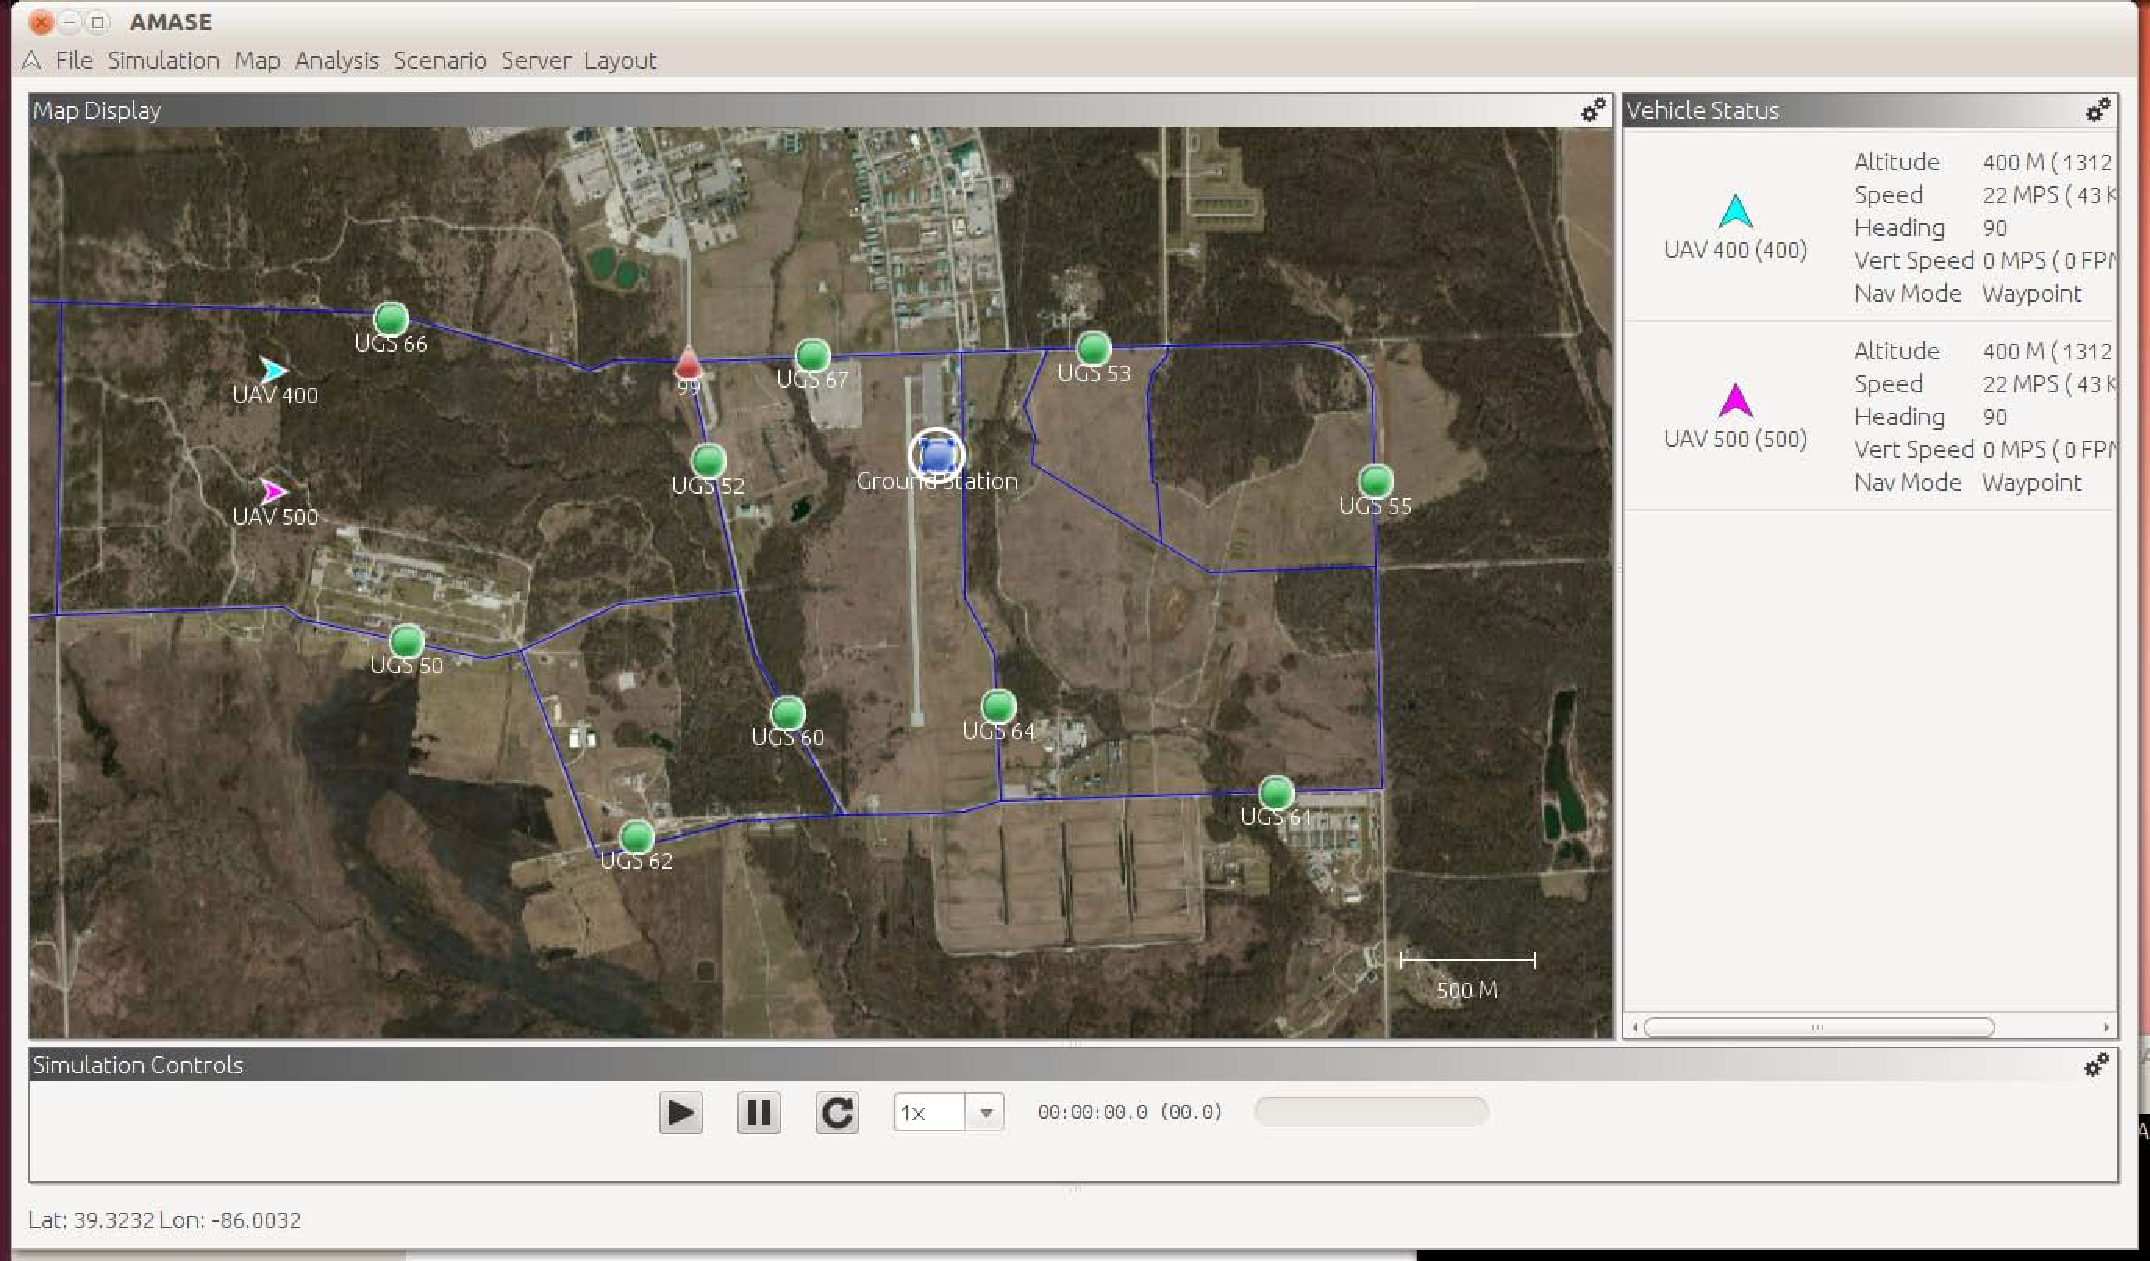
\includegraphics[width=1.3\linewidth]{\FiguresPath//AMASE_UGS_Scenario}
	\caption{AMASE simulation snapshot.}
	\label{fig:AMASE_Simulation_Snapshot}
\end{marginfigure}


The AMASE simulation is used to simulate the UxAS scenarios, see Figure \ref{fig:AMASE_Simulation_Snapshot}. AMASE was developed by members of AFRL's Aerospace Vehicles Technology Assessment \& Simulation Branch (AVTAS) to provide a common framework for research and development of cooperative control algorithms. AMASE was extended for UxAS in order to simulate \emph{communications} and \emph{on-board data processing}. AMASE includes the capability to connect to external programs using TCP/IP connections and LMCP messages. LMCP was developed by AFRL researchers to allow communication between cooperative control algorithms, ground stations, and simulations.

AMASE is written in Java to make it cross-platform compatible. It consists of a graphical front-end that displays simulated objects, a user interface to control the simulation, simulated air and ground vehicles,   and simulated communications. It has built-in, configurable, vehicle simulation models that are capable of following waypoint paths. AMASE uses the same LMCP messages as UxAS which makes it easy to communicate between the two. 

Communication between AMASE and other programs is implemented through TCP/IP connections. When a program (UxAS) connects to AMASE's general connection (port 55555), the program sends LMCP messages, such as \textit{MissionCommand}, to command the simulated vehicle's actions. AMASE sends all generated messages, such as \textit{AirVehicleStates}, to all connected programs (UxAS). In this manner, every connected program communicates with all of the entities in the simulation. There are also customization connections that make it possible to connect directly to simulated entities. These direct connections pass, only the messages that are available to the simulated entity, from AMASE to the external program (UXAS) . This makes it possible to connect multiple copies of UxAS to AMASE as if they are installed on-board the entities. This facilitates software-in-the-loop simulations.

\subsection{Working With AMASE}
The code for AMASE is located in the folder:
\begin{docspec}
    \textit{uxas/tools/amase/}
\end{docspec}
This folder contains three folders:
\begin{description}
\item[\textbf{\textit{AMASE\_DK/}}] contains the AMASE Development Kit, which is the core  executable software and documentation for AMASE.
\item[\textbf{\textit{amase-icet/}}] contains code that implements new functionality for UxAS-type projects. UxAS examples execute AMASE from this folder.  
\item[\textbf{\textit{amase-icet-lmcp/}}] contains the LMCP Java api generated to match the MDMs used by UxAS.
\end{description}

An AMASE simulation is configured by reading in a scenario file. These files use xml to define elements such as vehicle configurations, initial vehicle states, and initial vehicle commands. The file:
\begin{docspec}
	uxas/tools/amase/amase-icet/Scenario\_WaterwaySearch.xml
\end{docspec}
is an example of a scenario file that configures two simulated UAVs. The scenario file can be loaded at run-time or after starting AMASE, from the menu:
\begin{docspec}
	file->OpenScenario
\end{docspec}
Many elements of the simulation are optional and are configured using files in the folder:
\begin{docspec}
	uxas/tools/amase/amase-icet/config/communications/
\end{docspec}
These files include:
\begin{description}
\item[\textbf{EntityControl.xml}] - defines which models are used to make up the entity simulations. The port that are used to communicate directly to an entity are configure in this file. 
\item[\textbf{EntityIcons.xml}] maps type of entity to the icon used to represent it.
\item[\textbf{Plugins.xml}] contains entries for configuring plug-ins. For example, the different layers used in the maps are configured in this file. 
\item[\textbf{WindowService.xml}] configure layout and functionality of the windows in the AMASE user interface.
\end{description}

\newthought{Configuring Communication Ports}\\
By default the AMASE TCP/IP server is configured to connect on port \textbf{\textit{5555}}. This is configured in the \textit{Plugins.xml} file. Any client that connects to the \textit{localhost}, or the local IP address, on port \textbf{\textit{5555}} will receive all message generated in AMASE. Any messages sent to this port will be available to all entities in AMASE.

In order to run UxAS as if it is on-board the simulated UAVs, new connection types were implemented that form a connection from UxAS to the simulated UAVs. AMASE sends only information available to the connected UAV to UxAS. Any messages sent from UxAS are delivered only to the connected UAV.

These connections are configured in the file \textit{EntityControl.xml}. Here is a sample entry:
\begin{docspec}
<TcpConnection Id="100" Port="9100" />
\end{docspec}
The value of \textit{\textit{Id}} is the AMASE entity ID and the value of \textbf{\textit{Port}} is the port address of the connection.

\newthought{Using NASA Worldwind Maps}




\subsection{Running AMASE Step-by-Step}
\begin{enumerate}
\item open a terminal window in the folder:
\begin{docspec}
    \textit{uxas/tools/amase/}
\end{docspec}
\item start the bash script:
\begin{docspec}
    \textit{./runAMASE\_Sample.sh}
\end{docspec}
\item the AMASE user interface will open
\item push the "play" button to start the simulation
\end{enumerate}
This starts the AMASE simulation with the scenario file:
\begin{docspec}
    \textit{Scenario\_Sample.xml}
\end{docspec}
The command line in the bash script is:
\begin{docspec}
\textit{java -Xmx2048m -splash:./data/amase\_splash.png -classpath ./dist/*:./dist/lib/*  avtas.app.Application --config config/communications --scenario "Scenario\_Sample.xml";}
\end{docspec}

In order to facilitate running AMASE from the same folders as UxAS, the following bash script was developed to start AMSE:
\begin{fullwidth}
\begin{docspec}
here=\$PWD;\\
cd ../../tools/amase/amase-icet;\\
java -Xmx2048m -splash:./data/amase\_splash.png -classpath ./dist/*:./dist/lib/*  avtas.app.Application --config config/communications --scenario "Scenario\_WaterwaySearch.xml";\\
cd "\$here";
\end{docspec}
\end{fullwidth}


\subsection{Connecting UxAS to AMASE}
Connections from UxAS to AMASE entities requires UxAS to connect as a TCP/IP client. To accomplish this, a \textbf{\textit{LmcpObjectNetworkTcpBridge}} bridge (service) entry is needed in the UxAS config file. As an example, the following is the entry from the Waterway Search example:

\begin{fullwidth}
\begin{docspec}
    <Bridge Type="LmcpObjectNetworkTcpBridge" TcpAddress="tcp://127.0.0.1:5555" Server="FALSE">\\
        \quad <SubscribeToMessage MessageType="afrl.cmasi.MissionCommand" />\\
        \quad <SubscribeToMessage MessageType="afrl.cmasi.LineSearchTask" />\\
        \quad <SubscribeToMessage MessageType="afrl.cmasi.VehicleActionCommand" />\\
    </Bridge>
\end{docspec}
\end{fullwidth}
In this case UxAS is connecting to the general \textbf{\textit{5555}} connection. Any \textit{MissionCommand}, \textit{LineSerachTask}, or \textit{VehicleActionCommand} messages generated in UxAS will be sent to all of the entities in AMASE.

\newthought{Simulation Time}\\
AMASE is a simulation that generates its own time. UxAS time is based on the real-time clock. This can pose problems for complex UxAS services that rely on temporal synchronization. In order to address this problem, the service \textbf{\textit{Test\_SimulationTime}} was implemented. It is configured in the following manner:
\begin{docspec}
<Service Type="Test\_SimulationTime"/>
\end{docspec}
The \textbf{\textit{Test\_SimulationTime}} service switches UxAS to \textit{discrete-time} mode. It subscribes to \textit{AirVehicleState} messages and when it receives one, it sets UxAS time equal to the time contained in the \textit{AirVehicleState}. As AMASE runs it sends out \textit{AirVehicleState} messages with the current simulation time which makes it possible to synchronize UxAS. 

%\cite{Duquette:2010}